\documentclass[12pt,a4paper,oneside,brazil,chapter=TITLE,section=TITLE]{abntex2}

%% Pacotes
\usepackage[T1]{fontenc}
\usepackage[utf8]{inputenc}
\usepackage[brazil]{babel}
\usepackage{lmodern}
\usepackage{microtype}
\usepackage{graphicx}
\usepackage{amsmath,amssymb}
\usepackage{booktabs}
\usepackage{float}
\usepackage{listings}
\usepackage{xcolor}
\usepackage{caption}
\usepackage{subcaption}
\usepackage{geometry}
\usepackage{abntex2cite}
\usepackage{url}

\geometry{top=3cm,bottom=2cm,left=3cm,right=2cm}

%% Listagens
\lstset{
  basicstyle=\ttfamily\footnotesize,
  breaklines=true,
  keywordstyle=\color{blue!70!black}\bfseries,
  commentstyle=\color{green!50!black}\itshape,
  stringstyle=\color{red!60!black},
  numbers=left, numberstyle=\tiny\color{gray},
  numbersep=6pt,
  frame=single, rulecolor=\color{gray!40},
  tabsize=2,
  showstringspaces=false,
  literate={>=}{{\(\geq\)}}1 {<=}{{\(\leq\)}}1,
}
\lstdefinestyle{matlab}{language=Matlab}
\lstdefinestyle{python}{language=Python}

%% Metadados
\titulo{Projeto 9 -- Filtros Butterworth e Filtro de Alta \^Enfase}
\autor{Matheus Serr\~ao Uch\^oa}
\local{Manaus -- AM}
\data{maio de 2026}
\instituicao{%
  Universidade Federal do Amazonas -- UFAM\\
  Instituto de Computa\c{c}\~ao -- IComp\\
  Disciplina: Processamento Digital de Imagens}
\tipotrabalho{Relat\'orio de Atividade}
\preambulo{Relat\'orio referente ao Projeto~9 da disciplina de
  Processamento Digital de Imagens, abordando filtros passa-baixa e
  passa-alta de Butterworth no dom\'inio da frequ\^encia e implementa\c{c}\~ao
  do Filtro de Alta \^Enfase (\textit{High-Emphasis Filter}).}

%% PDF metadata
\makeatletter
\hypersetup{
  pdftitle={\@titulo},
  pdfauthor={\@autor},
  colorlinks=true,
  linkcolor=blue!60!black,
  citecolor=green!50!black,
  urlcolor=blue
}
\makeatother

\begin{document}

%% ================================================================
%% CAPA
%% ================================================================
\begin{capa}
  \center
  
\includegraphics[width=3cm]{ufam_logo.png}\\[0.5cm]
  {\large\bfseries Universidade Federal do Amazonas}\\
  {\large Instituto de Computa\c{c}\~ao -- IComp}\\[1cm]
  \vfill
  {\LARGE\bfseries Processamento Digital de Imagens}\\[0.4cm]
  {\Large\bfseries Projeto 9}\\[0.3cm]
  {\large Filtros Butterworth e Filtro de Alta \^Enfase}\\
  \vfill
  {\large Matheus Serr\~ao Uch\^oa}\\[0.5cm]
  {\large Manaus -- AM, maio de 2026}
\end{capa}

%% ================================================================
%% FOLHA DE ROSTO
%% ================================================================
\begin{folhaderosto}
  \begin{center}
    {\large\bfseries Matheus Serr\~ao Uch\^oa}\\[2cm]
    {\LARGE\bfseries Projeto 9 -- Filtros Butterworth\\e Filtro de Alta \^Enfase}\\[1.5cm]
  \end{center}

  \begin{flushright}
    \begin{minipage}{9cm}
      \small
      Relat\'orio apresentado como atividade avaliativa da disciplina
      de Processamento Digital de Imagens do Instituto de Computa\c{c}\~ao
      da Universidade Federal do Amazonas.
    \end{minipage}
  \end{flushright}

  \vfill
  \begin{center}
    {\large Manaus -- AM, maio de 2026}
  \end{center}
\end{folhaderosto}

%% ================================================================
%% RESUMO
%% ================================================================
\begin{resumo}
Este relat\'orio descreve a implementa\c{c}\~ao e avalia\c{c}\~ao de
filtros no dom\'inio da frequ\^encia aplicados ao processamento digital
de imagens. Na Parte~(a), s\~ao aplicados filtros passa-baixa e
passa-alta de Butterworth \`a imagem \textit{woman.tif}, com visualiza\c{c}\~ao
2D e 3D dos filtros e do espectro centralizado de Fourier.
Na Parte~(b), \'e implementada a fun\c{c}\~ao
\texttt{highEnphasisFilt}, que realiza a filtragem de alta \^enfase
(\textit{High-Emphasis Filter} -- HEF) combinando um offset com a
resposta em frequ\^encia passa-alta de Butterworth.
Na Parte~(c), o filtro HEF \'e aplicado \`a imagem \textit{chestXray.tif}
(radiografia de t\'orax), seguido de equaliza\c{c}\~ao de histograma,
evidenciando o realce de bordas e detalhes finos em imagens m\'edicas.
Os resultados demonstram que o HEF preserva as baixas frequ\^encias
enquanto amplifica as altas, melhorando a nitidez e o contraste.

\vspace{0.5cm}
\noindent\textbf{Palavras-chave:}
Filtro de Butterworth.
Passa-baixa.
Passa-alta.
Filtro de Alta \^Enfase.
Dom\'inio da frequ\^encia.
Equaliza\c{c}\~ao de histograma.
\end{resumo}

%% ================================================================
%% SUMARIO
%% ================================================================
\tableofcontents*
\cleardoublepage

%% ================================================================
%% TEXTUAL
%% ================================================================
\textual

%% ----------------------------------------------------------------
\chapter{Introdu\c{c}\~ao}
%% ----------------------------------------------------------------

A filtragem no dom\'inio da frequ\^encia \'e uma das ferramentas
fundamentais do processamento digital de imagens (PDI).
Ao operar no espa\c{c}o de Fourier, \'e poss\'ivel projetar respostas
em frequ\^encia arbitr\'arias com grande controle sobre as
caracter\'isticas de corte e transi\c{c}\~ao, o que \'e dif\'icil
de obter com filtros espaciais convencionais.

O filtro de Butterworth \cite{gonzalez2018} destaca-se por apresentar
resposta maximamente plana na banda de passagem e transi\c{c}\~ao
suave entre bandas, evitando os artefatos de oscila\c{c}\~ao
(\textit{ringing}) caracter\'isticos do filtro ideal
\cite{oppenheim1999}.
O Filtro de Alta \^Enfase (\textit{High-Emphasis Filter} -- HEF)
\'e uma extens\~ao que permite preservar a ilumina\c{c}\~ao geral
da cena enquanto amplifica as altas frequ\^encias associadas a bordas
e texturas \cite{gonzalez2018}.

Este relat\'orio est\'a organizado em tr\^es partes:
\begin{itemize}
  \item \textbf{Parte (a):} aplica\c{c}\~ao de filtros PB e PA de
        Butterworth na imagem \textit{woman.tif}, com an\'alise do
        espectro de Fourier centralizado;
  \item \textbf{Parte (b):} implementa\c{c}\~ao da fun\c{c}\~ao
        \texttt{highEnphasisFilt} em MATLAB com visualiza\c{c}\~ao
        2D/3D;
  \item \textbf{Parte (c):} aplica\c{c}\~ao do HEF \`a radiografia
        de t\'orax \textit{chestXray.tif} e equaliza\c{c}\~ao de
        histograma.
\end{itemize}

%% ----------------------------------------------------------------
\chapter{Fundamenta\c{c}\~ao Te\'orica}
%% ----------------------------------------------------------------

\section{Transformada de Fourier Discreta Bidimensional}

Dada uma imagem $f(x,y)$ de tamanho $M \times N$, sua Transformada de
Fourier Discreta (DFT) \'e definida como:
\begin{equation}
  F(u,v) = \sum_{x=0}^{M-1}\sum_{y=0}^{N-1}
            f(x,y)\,e^{-j2\pi(ux/M + vy/N)},
\end{equation}
onde $u = 0, 1, \ldots, M-1$ e $v = 0, 1, \ldots, N-1$.
A centraliza\c{c}\~ao do espectro, obtida via \texttt{fftshift}, desloca
as frequ\^encias zero para o centro da imagem, facilitando a visualiza\c{c}\~ao
e o projeto de filtros com simetria circular.

A filtragem no dom\'inio da frequ\^encia segue o teorema da
convolu\c{c}\~ao:
\begin{equation}
  G(u,v) = H(u,v) \cdot F(u,v),
\end{equation}
onde $H(u,v)$ \'e a fun\c{c}\~ao de transfer\^encia do filtro.
A imagem filtrada \'e obtida pela DFT inversa:
\begin{equation}
  g(x,y) = \mathcal{F}^{-1}\{G(u,v)\}.
\end{equation}

\section{Filtro de Butterworth}

A dist\^ancia entre um ponto $(u,v)$ e o centro do espectro \'e:
\begin{equation}
  D(u,v) = \sqrt{u^2 + v^2}.
\end{equation}

O filtro passa-baixa (PB) de Butterworth de ordem $n$ e frequ\^encia
de corte $D_0$ \'e definido por:
\begin{equation}
  H_{\text{LP}}(u,v) = \frac{1}{1 + \left[D(u,v)/D_0\right]^{2n}}.
  \label{eq:blp}
\end{equation}

O filtro passa-alta (PA) correspondente \'e obtido por:
\begin{equation}
  H_{\text{HP}}(u,v) = 1 - H_{\text{LP}}(u,v).
  \label{eq:bhp}
\end{equation}

Para $D = D_0$, a resposta do filtro PB \'e $1/\sqrt{2} \approx 0{,}707$,
independentemente da ordem $n$.
Valores maiores de $n$ produzem transi\c{c}\~ao mais abrupta, aproximando
o comportamento do filtro ideal, por\'em aumentando o \textit{ringing}
na imagem espacial.

\section{Filtro de Alta \^Enfase}

O Filtro de Alta \^Enfase (HEF) combina um componente de corrente
cont\'inua com a amplifica\c{c}\~ao seletiva das altas frequ\^encias:
\begin{equation}
  H_{\text{HFE}}(u,v) = a + b \cdot H_{\text{HP}}(u,v),
  \label{eq:hef}
\end{equation}
onde:
\begin{itemize}
  \item $a \geq 0$: offset que garante a preserva\c{c}\~ao das baixas
        frequ\^encias (ilumina\c{c}\~ao geral);
  \item $b > 0$: fator de amplifica\c{c}\~ao das altas frequ\^encias
        (bordas e texturas).
\end{itemize}

Quando $a = 0$ e $b = 1$, o HEF reduz-se ao filtro PA puro.
Valores t\'ipicos $a \approx 0{,}5$ e $b \approx 2{,}0$ preservam
a imagem base e enfatizam os detalhes finos \cite{gonzalez2018}.

A equaliza\c{c}\~ao de histograma \cite{gonzalez2018}, aplicada ap\'os o HEF,
redistribui os n\'iveis de cinza de forma a maximizar o contraste global,
complementando o realce de bordas obtido pelo filtro.

%% ----------------------------------------------------------------
\chapter{Implementa\c{c}\~ao}
%% ----------------------------------------------------------------

\section{Parte (a) -- Filtros Butterworth em \textit{woman.tif}}

O c\'odigo principal \texttt{main\_project9.m} carrega a imagem
\textit{woman.tif}, computa a DFT centralizada e aplica os filtros
PB e PA de Butterworth com $D_0 = 60$ e $n = 2$.

\begin{lstlisting}[style=matlab, caption={Trecho principal -- Parte (a)}]
f_w = double(imread('imgs_orig/woman.tif'));
[rows, cols] = size(f_w);
D0 = 60; n = 2;

[U, V] = meshgrid(-(cols/2):(cols/2-1), -(rows/2):(rows/2-1));
D = sqrt(U.^2 + V.^2);

H_LP = 1 ./ (1 + (D ./ D0).^(2*n));
H_HP = 1 - H_LP;

F_w  = fftshift(fft2(f_w));
g_lp = real(ifft2(ifftshift(H_LP .* F_w)));
g_hp = real(ifft2(ifftshift(H_HP .* F_w)));
\end{lstlisting}

\section{Parte (b) -- Fun\c{c}\~ao \texttt{highEnphasisFilt}}

A fun\c{c}\~ao implementa a equa\c{c}\~ao~\eqref{eq:hef} aceitando os
par\^ametros $a$, $b$, a imagem $f$, o tipo de filtro, $D_0$, $n$ e uma
\textit{flag} de visualiza\c{c}\~ao.

\begin{lstlisting}[style=matlab,
  caption={highEnphasisFilt.m -- n\'ucleo do filtro}]
function [H, g] = highEnphasisFilt(a, b, f, type, D0, n, show)
  f = double(f);
  [rows, cols] = size(f);
  [U, V] = meshgrid(-(cols/2):(cols/2-1), -(rows/2):(rows/2-1));
  D = sqrt(U.^2 + V.^2);
  H_LP = 1 ./ (1 + (D ./ D0).^(2*n));
  H_HP = 1 - H_LP;
  H    = a + b * H_HP;
  F    = fftshift(fft2(f));
  g_raw = real(ifft2(ifftshift(H .* F)));
  g_min = min(g_raw(:)); g_max = max(g_raw(:));
  g = uint8(255 * (g_raw - g_min) / (g_max - g_min + eps));
end
\end{lstlisting}

\section{Parte (c) -- HEF e Equaliza\c{c}\~ao em \textit{chestXray.tif}}

Para a radiografia de t\'orax, os par\^ametros escolhidos foram
$D_0 = 40$, $n = 2$, $a = 0{,}5$ e $b = 2{,}0$.
Ap\'os a filtragem HEF, aplica-se \texttt{histeq} para maximizar o contraste.

\begin{lstlisting}[style=matlab,
  caption={Parte (c) -- HEF e equaliza\c{c}\~ao}]
f_c = double(imread('imgs_orig/chestXray.tif'));
[H_hfe_c, g_hfe_c] = highEnphasisFilt(0.5, 2.0, f_c,
                       'butterworth', 40, 2, false);
g_eq = histeq(g_hfe_c);
\end{lstlisting}

%% ----------------------------------------------------------------
\chapter{Resultados e Discuss\~ao}
%% ----------------------------------------------------------------

\section{Parte (a) -- Espectro e Filtros Butterworth}

A Figura~\ref{fig:part_a_overview} apresenta, da esquerda para a direita:
a imagem original \textit{woman.tif}, o espectro $\log(1+|F|)$ centralizado,
o filtro PB visualizado em 2D, a imagem filtrada pelo PB, o espectro
resultante e a imagem filtrada pelo PA.

\begin{figure}[H]
  \centering
  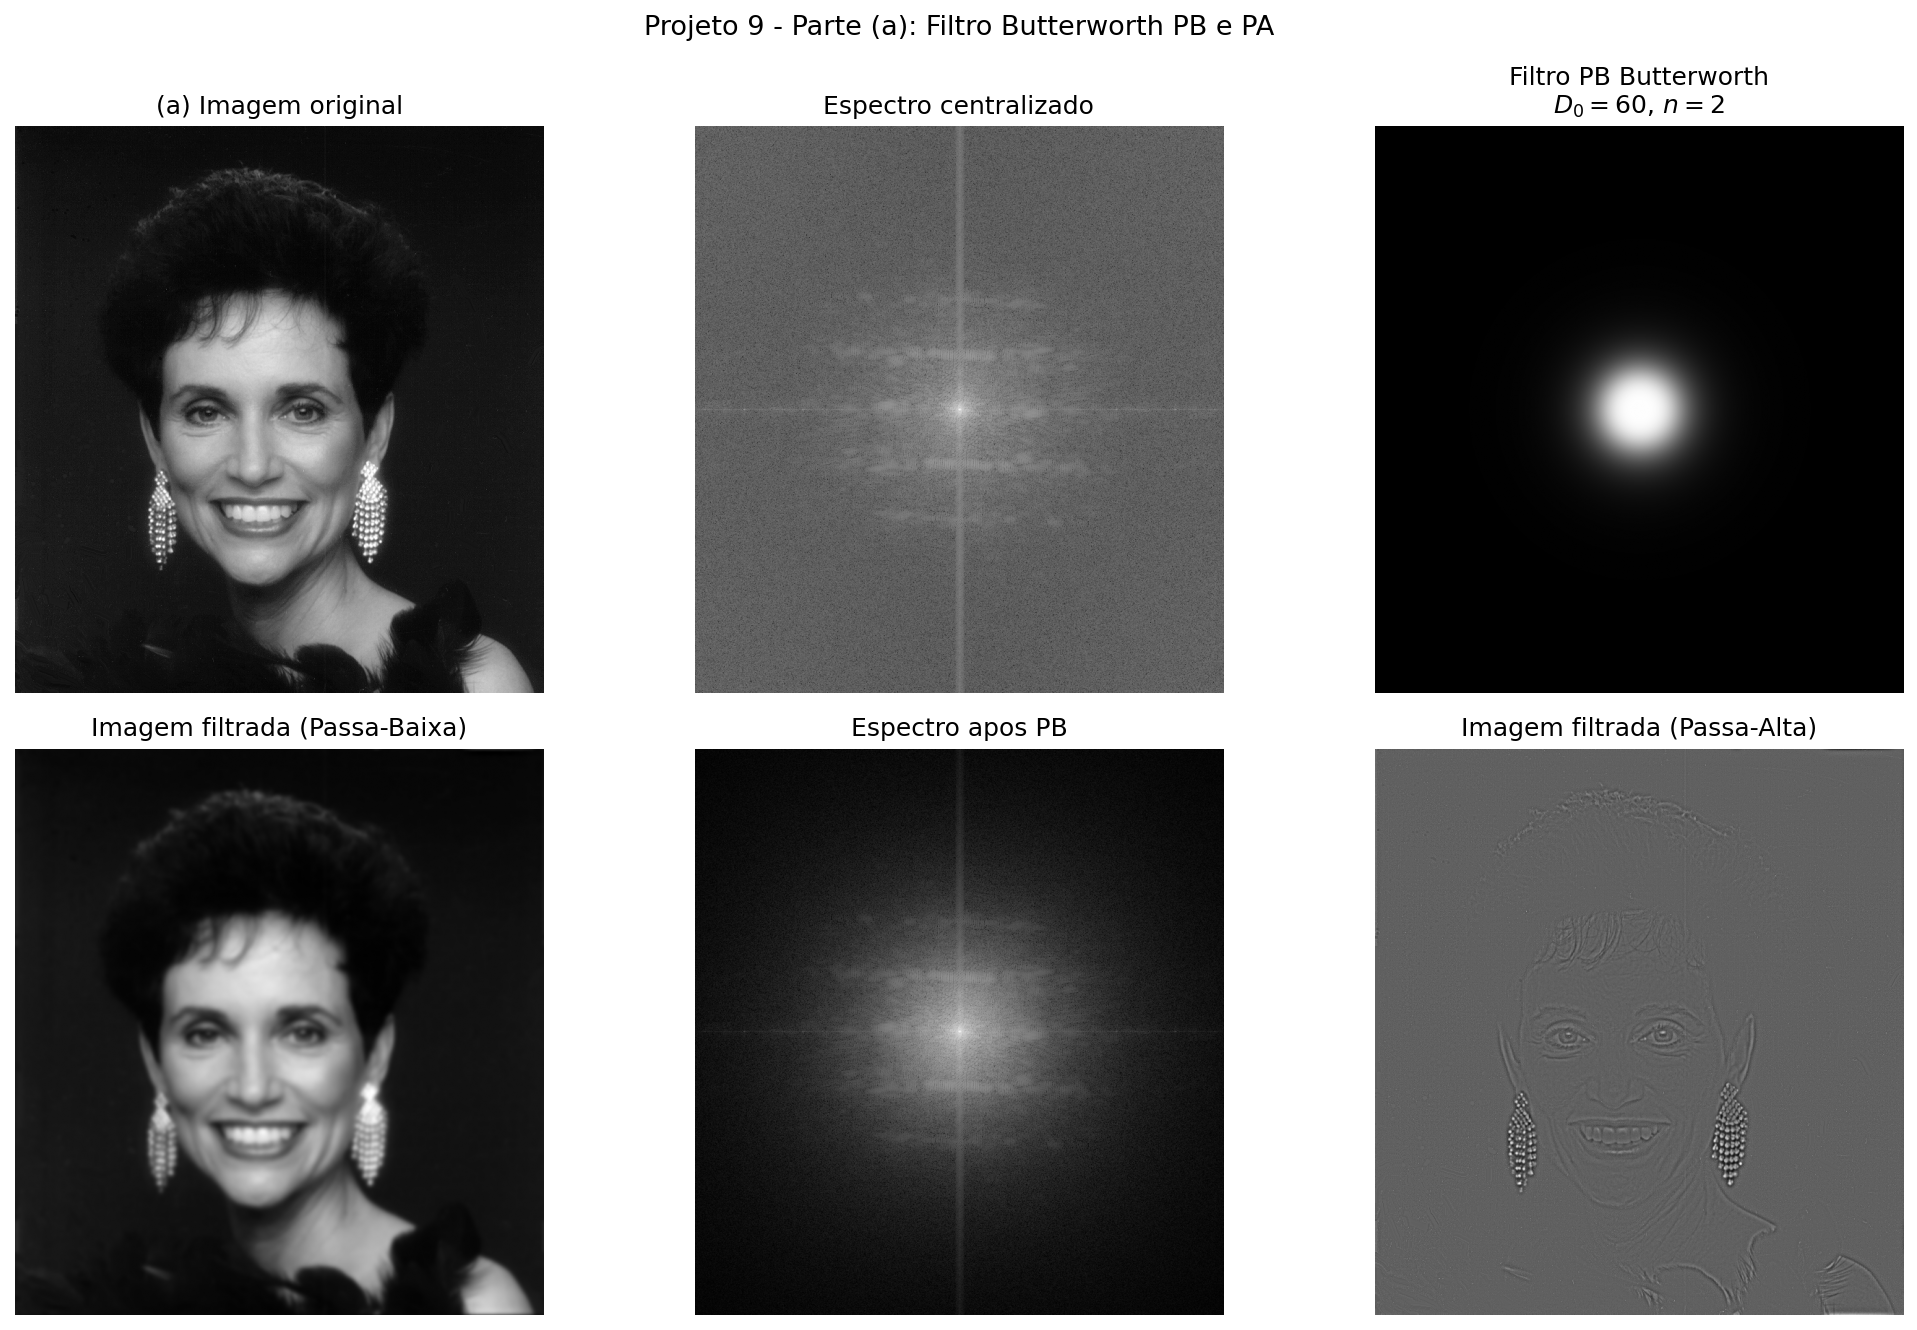
\includegraphics[width=\linewidth]{imgs_result/part_a_results.png}
  \caption{Parte (a): imagem original, espectro de Fourier centralizado,
           filtro PB Butterworth 2D, resultado PB, espectro PB e resultado PA.
           $D_0 = 60$, $n = 2$.}
  \label{fig:part_a_overview}
  \fonte{Elaborado pelo autor (2026).}
\end{figure}

O espectro centralizado exibe a concentra\c{c}\~ao de energia nas baixas
frequ\^encias (regi\~ao central), enquanto as altas frequ\^encias
(bordas, texturas) ficam distribu\'idas na periferia.
O filtro PB suaviza a imagem eliminando as altas frequ\^encias, e o
filtro PA realca as bordas suprimindo as baixas frequ\^encias.

As Figuras~\ref{fig:part_a_lp_3d} e~\ref{fig:part_a_hp_3d} mostram as
visualiza\c{c}\~oes 3D dos filtros PB e PA, respectivamente.

\begin{figure}[H]
  \centering
  \begin{subfigure}[b]{0.48\linewidth}
    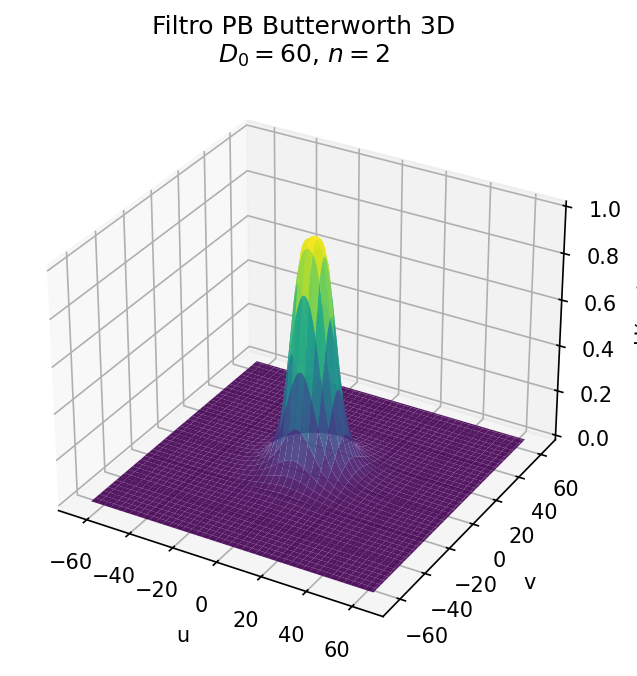
\includegraphics[width=\linewidth]{imgs_result/part_a_lp_3d.png}
    \caption{Filtro PB 3D ($D_0 = 60$, $n = 2$).}
    \label{fig:part_a_lp_3d}
  \end{subfigure}\hfill
  \begin{subfigure}[b]{0.48\linewidth}
    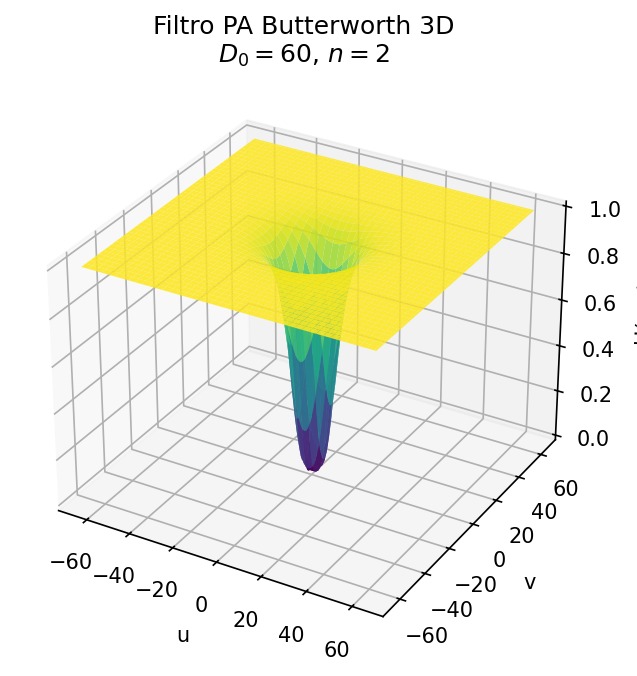
\includegraphics[width=\linewidth]{imgs_result/part_a_hp_3d.png}
    \caption{Filtro PA 3D ($D_0 = 60$, $n = 2$).}
    \label{fig:part_a_hp_3d}
  \end{subfigure}
  \caption{Visualiza\c{c}\~ao 3D dos filtros Butterworth.}
  \fonte{Elaborado pelo autor (2026).}
\end{figure}

A visualiza\c{c}\~ao 3D evidencia a transi\c{c}\~ao suave caracter\'istica
do filtro de Butterworth: n\~ao h\'a descontinuidade abrupta em $D_0$,
o que minimiza os artefatos de \textit{ringing} na imagem filtrada.
Para $n = 2$, a transi\c{c}\~ao \'e moderada; ordens maiores produziriam
uma queda mais acentuada pr\'oxima a $D_0$.

\begin{figure}[H]
  \centering
  \begin{subfigure}[b]{0.48\linewidth}
    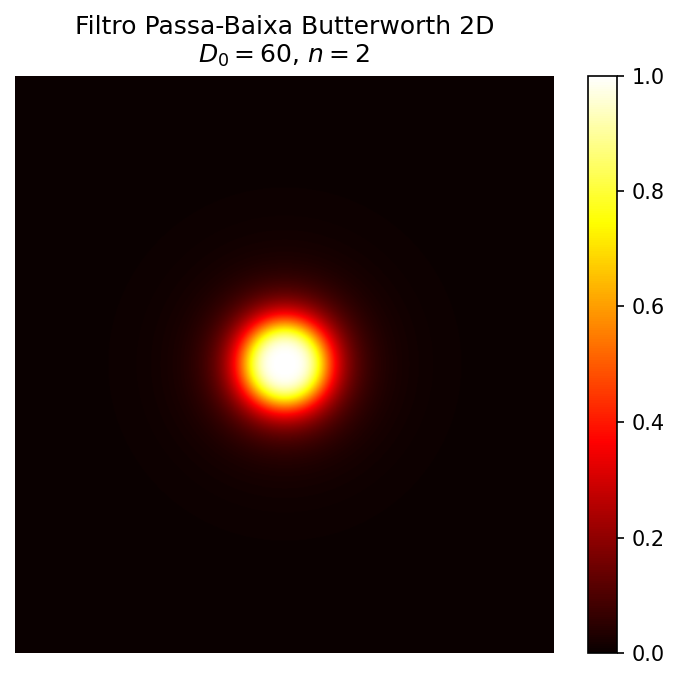
\includegraphics[width=\linewidth]{imgs_result/part_a_lp_2d.png}
    \caption{Filtro PB 2D.}
  \end{subfigure}\hfill
  \begin{subfigure}[b]{0.48\linewidth}
    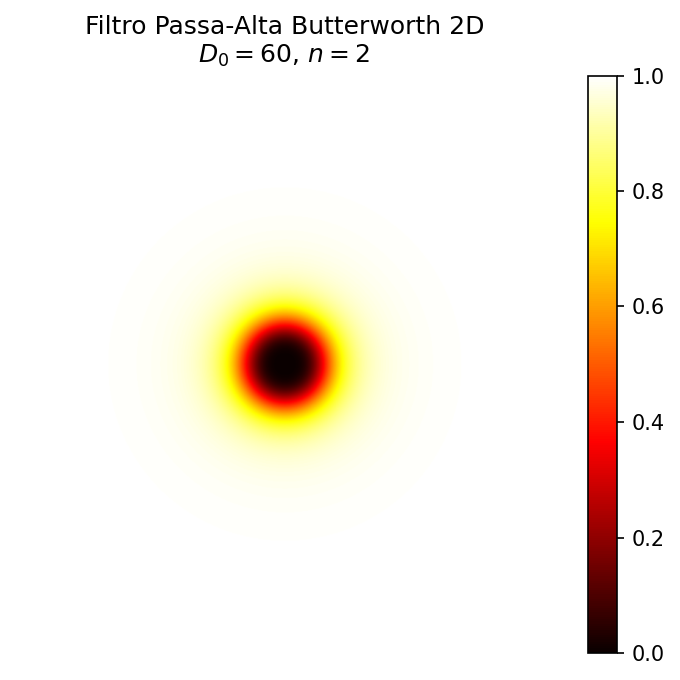
\includegraphics[width=\linewidth]{imgs_result/part_a_hp_2d.png}
    \caption{Filtro PA 2D.}
  \end{subfigure}
  \caption{Visualiza\c{c}\~ao 2D dos filtros Butterworth ($D_0 = 60$, $n = 2$).}
  \fonte{Elaborado pelo autor (2026).}
\end{figure}

\section{Parte (b) -- Filtro de Alta \^Enfase}

A Figura~\ref{fig:part_b_hef2d} apresenta o filtro HEF em 2D e em
detalhe, e a Figura~\ref{fig:part_b_hef3d} mostra sua visualiza\c{c}\~ao
3D.

\begin{figure}[H]
  \centering
  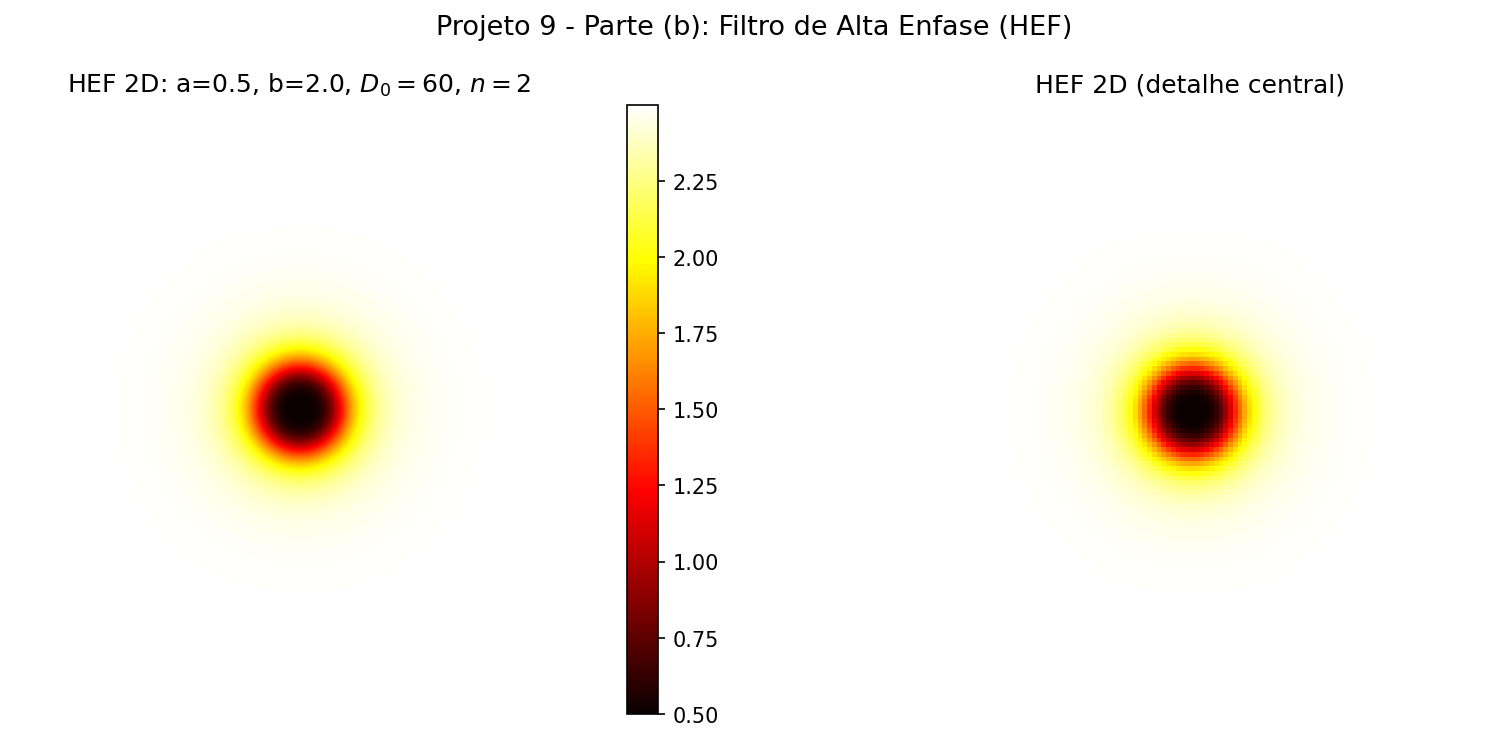
\includegraphics[width=\linewidth]{imgs_result/part_b_hef_2d.png}
  \caption{Filtro HEF 2D: $a=0{,}5$, $b=2{,}0$, $D_0=60$, $n=2$.
           A escala de cores mostra que as baixas frequ\^encias
           t\^em ganho $a = 0{,}5$ e as altas atingem $a + b = 2{,}5$.}
  \label{fig:part_b_hef2d}
  \fonte{Elaborado pelo autor (2026).}
\end{figure}

\begin{figure}[H]
  \centering
  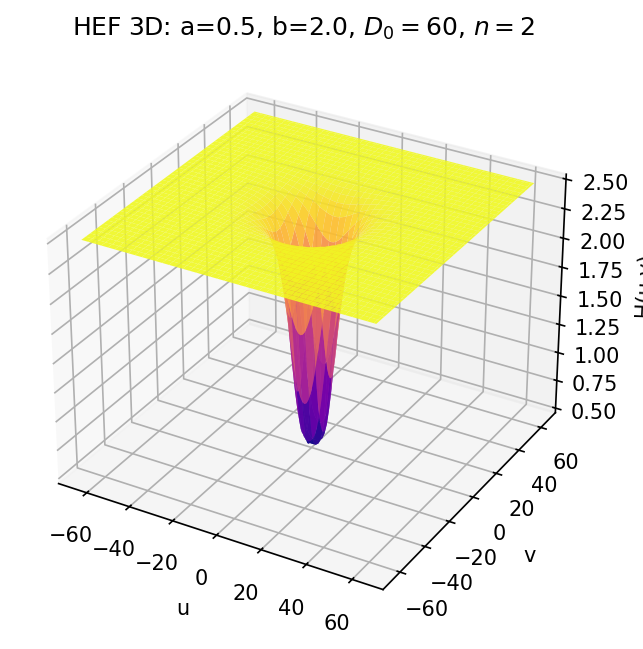
\includegraphics[width=0.6\linewidth]{imgs_result/part_b_hef_3d.png}
  \caption{Visualiza\c{c}\~ao 3D do filtro HEF.}
  \label{fig:part_b_hef3d}
  \fonte{Elaborado pelo autor (2026).}
\end{figure}

A Figura~\ref{fig:part_b_woman} compara a imagem original com o resultado
do HEF, evidenciando o realce de bordas e texturas finas preservando a
ilumina\c{c}\~ao geral.

\begin{figure}[H]
  \centering
  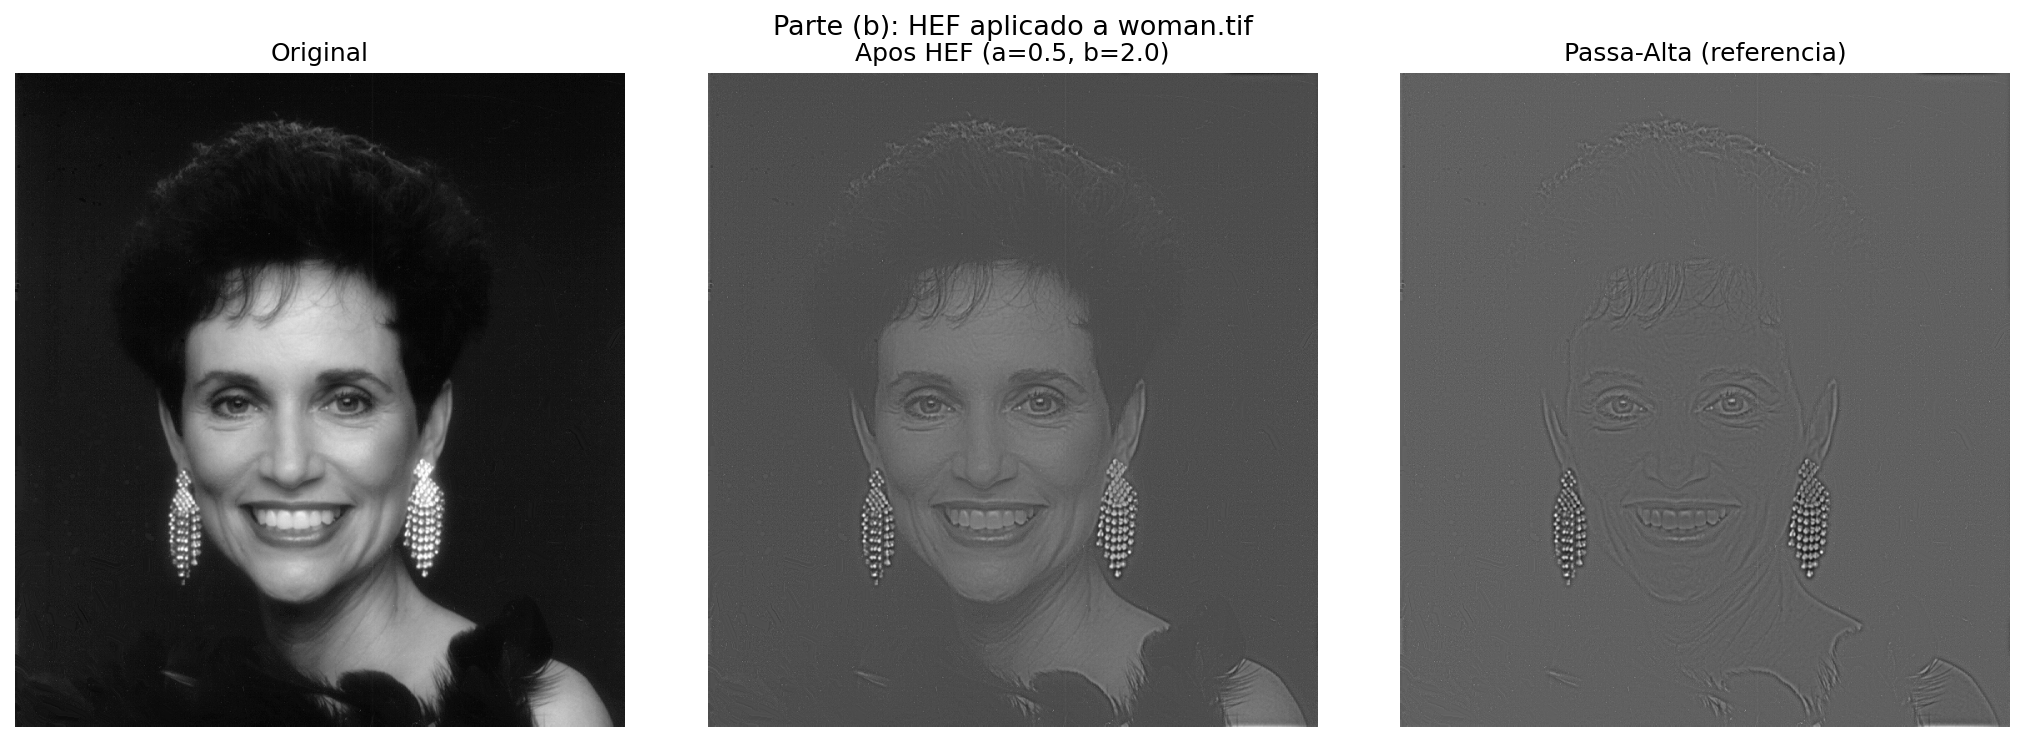
\includegraphics[width=\linewidth]{imgs_result/part_b_woman_hef.png}
  \caption{Parte (b): original, resultado HEF e filtro PA de
           refer\^encia em \textit{woman.tif}.}
  \label{fig:part_b_woman}
  \fonte{Elaborado pelo autor (2026).}
\end{figure}

\noindent\textbf{Compara\c{c}\~ao com o PA puro:} enquanto o filtro PA
($a=0$, $b=1$) elimina a componente DC produzindo uma imagem
predominantemente de bordas, o HEF com $a=0{,}5$ mant\'em a estrutura
geral da cena. O valor $b=2$ dobra a contribui\c{c}\~ao das altas
frequ\^encias em rela\c{c}\~ao \`as baixas, resultando em nitidez
notavelmente superior sem perda da informa\c{c}\~ao tonal.

\section{Parte (c) -- HEF e Equaliza\c{c}\~ao em Radiografia de T\'orax}

A Figura~\ref{fig:part_c_main} resume a cadeia de processamento aplicada
\`a imagem \textit{chestXray.tif}.

\begin{figure}[H]
  \centering
  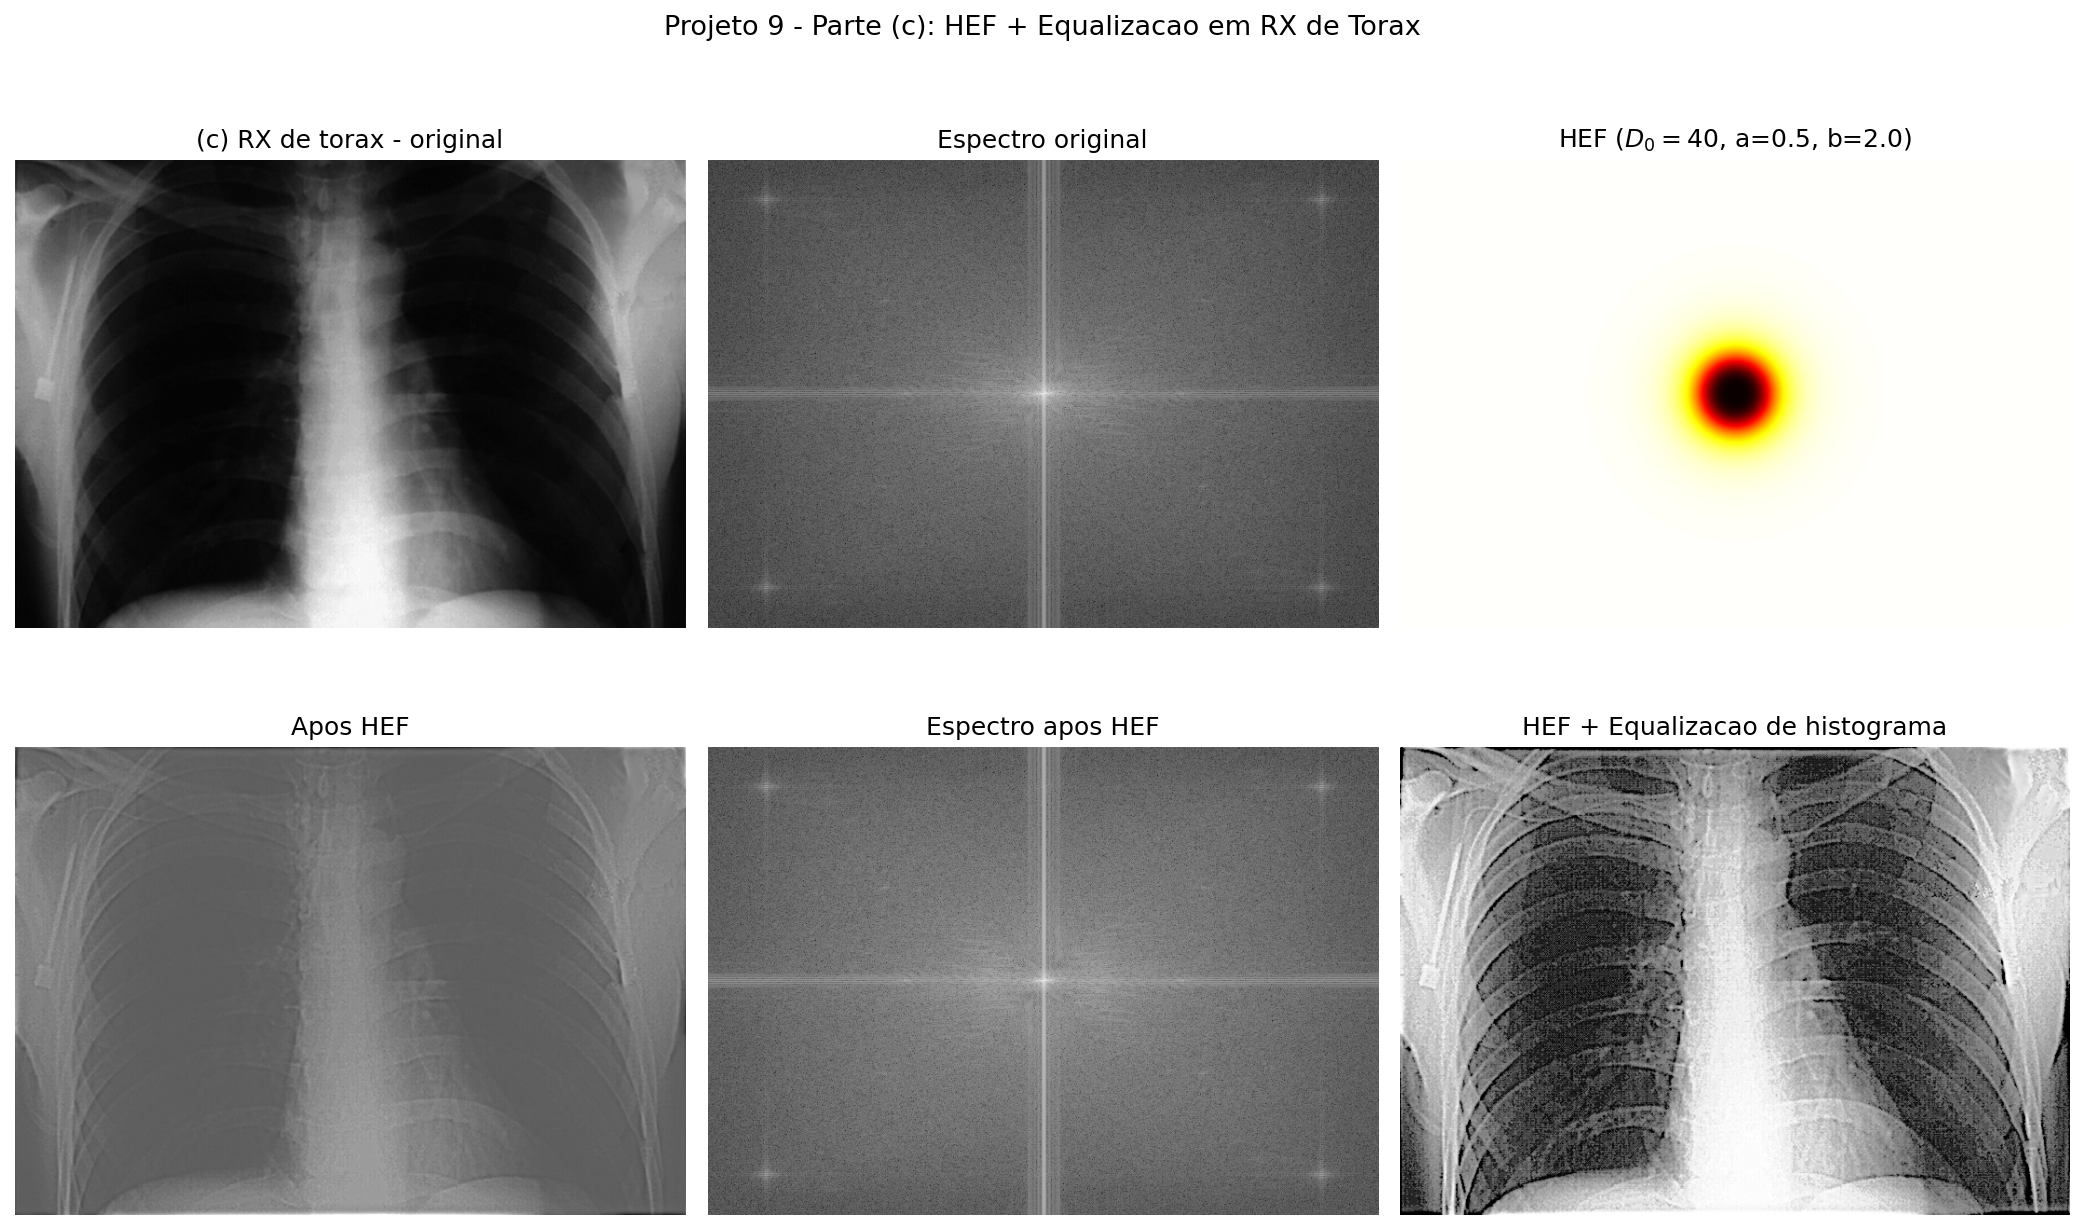
\includegraphics[width=\linewidth]{imgs_result/part_c_chest_results.png}
  \caption{Parte (c): imagem original, espectro original, filtro HEF,
           imagem ap\'os HEF, espectro ap\'os HEF e resultado final
           (HEF + equaliza\c{c}\~ao de histograma).}
  \label{fig:part_c_main}
  \fonte{Elaborado pelo autor (2026).}
\end{figure}

A compara\c{c}\~ao dos espectros (Figura~\ref{fig:part_c_spectra}) confirma
que o HEF amplifica as altas frequ\^encias: o espectro filtrado exibe
energia maior na regi\~ao perif\'erica, que corresponde \`as estruturas
finas do tecido pulmonar e \`as bordas das costelas.

\begin{figure}[H]
  \centering
  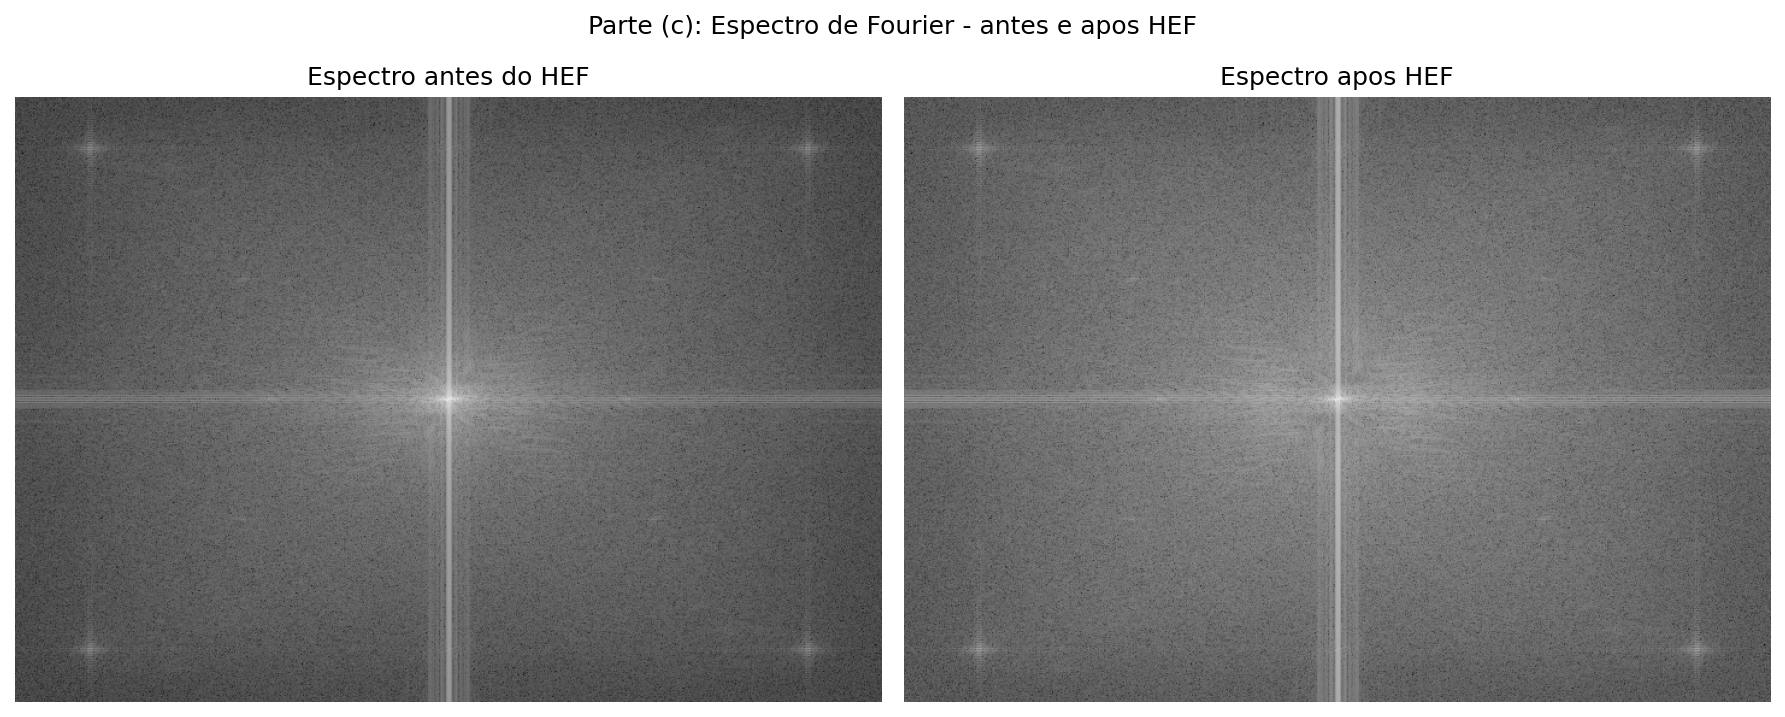
\includegraphics[width=\linewidth]{imgs_result/part_c_spectra_comparison.png}
  \caption{Espectro de Fourier antes e ap\'os o HEF em
           \textit{chestXray.tif}.}
  \label{fig:part_c_spectra}
  \fonte{Elaborado pelo autor (2026).}
\end{figure}

A Figura~\ref{fig:part_c_hist} apresenta os histogramas das tr\^es etapas.
A imagem original apresenta distribui\c{c}\~ao concentrada nas m\'edias
intensidades. Ap\'os o HEF, o histograma alarga-se levemente.
A equaliza\c{c}\~ao de histograma redistribui uniformemente os n\'iveis,
maximizando o contraste e tornando vis\'iveis detalhes que estavam encobertos.

\begin{figure}[H]
  \centering
  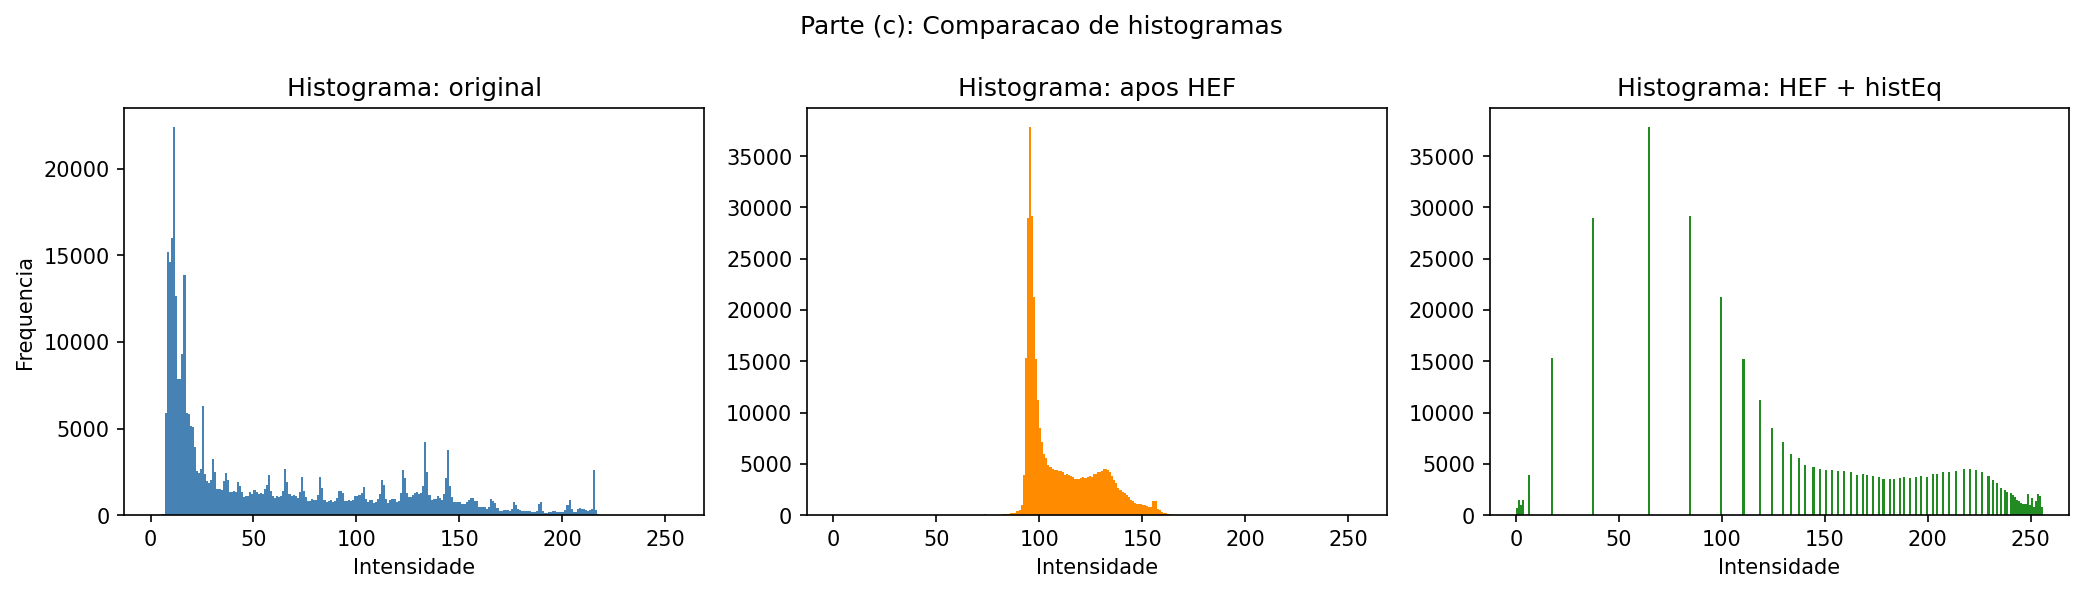
\includegraphics[width=\linewidth]{imgs_result/part_c_histograms.png}
  \caption{Histogramas: original, ap\'os HEF e ap\'os HEF + equaliza\c{c}\~ao.}
  \label{fig:part_c_hist}
  \fonte{Elaborado pelo autor (2026).}
\end{figure}

\noindent\textbf{Discuss\~ao cl\'inica:} em imagens de raio-X, o realce
de bordas melhora a visualiza\c{c}\~ao de n\'odulos pulmonares, pneumonia
e outras patologias de baixo contraste. A combina\c{c}\~ao HEF $+$
equaliza\c{c}\~ao de histograma \'e uma t\'ecnica cl\'assica de
pr\'e-processamento em sistemas de aux\'ilio ao diagn\'ostico por imagem
(CAD) \cite{gonzalez2018}.

%% ----------------------------------------------------------------
\chapter{Conclus\~ao}
%% ----------------------------------------------------------------

Este trabalho demonstrou a aplica\c{c}\~ao de filtros no dom\'inio da
frequ\^encia para o realce de imagens digitais.
Os principais resultados obtidos foram:

\begin{enumerate}
  \item O filtro passa-baixa de Butterworth suaviza a imagem de forma
        gradual, sem artefatos de \textit{ringing}, enquanto o filtro
        passa-alta realca bordas e texturas;
  \item O Filtro de Alta \^Enfase, implementado como
        $H_{\text{HFE}} = a + b \cdot H_{\text{HP}}$, permite controlar
        independentemente a preserva\c{c}\~ao da ilumina\c{c}\~ao ($a$)
        e a amplifica\c{c}\~ao das altas frequ\^encias ($b$);
  \item A aplica\c{c}\~ao em radiografia de t\'orax evidenciou a utilidade
        do HEF em imagens m\'edicas, onde a nitidez de bordas \'e
        cr\'itica para o diagn\'ostico;
  \item A equaliza\c{c}\~ao de histograma complementa o HEF ao redistribuir
        os n\'iveis de cinza, maximizando o contraste global da imagem
        resultante.
\end{enumerate}

O c\'odigo MATLAB entregue \'e gen\'erico e parametriz\'avel, permitindo
experimenta\c{c}\~ao com diferentes valores de $D_0$, $n$, $a$ e $b$
para outras aplica\c{c}\~oes.

%% ================================================================
%% POSTEXTUAL
%% ================================================================
\postextual
\bibliography{referencias_project9}

\end{document}
